%!TEX root = ../pres - final.tex

\section{Speaker Diarization}

\subsection{Formulación matemática}
\begin{frame}{Formulación matemática (I)}
  Denótese por $\mathcal{A}$ la \alert{evidencia acústica} a partir de la cuál el modelo deberá encontrar la segmentación correcta para un fragmento de señal.
  \\~\\
  Se puede pensar en $\mathcal{A}$ como la secuencia de símbolos correspondiente a un segmento de señal, y que está conformada por elementos de un alfabeto mucho más grande $\mathbb{A}$. 
  \begin{equation}
  \mathcal{A} = a_1, a_2, ..., a_K \quad a_i \in \mathbb{A}
  \label{eqn:2a-1}
  \end{equation}
  en donde los elementos $a_i$ hacen referencia a un intervalo de tiempo $i$ en la secuencia de audio original.
  %, y los valores que tomen pueden repetirse de acuerdo a la grabación.
  %\vfill
\end{frame}

\begin{frame}{Formulación matemática (II)}
  De la misma manera,
  \begin{equation}
  \mathcal{S} = s_1, s_2, ..., s_N \quad s_i \in \mathbb{S}
  \label{eqn:2a-2}
  \end{equation}
  donde $\mathcal{S}$ es la secuencia que corresponde a una \alert{propuesta de segmentación} para un intervalo del audio original. 
  \\~\\
  $\mathbb{S}$ es el conjunto de todos los interlocutores que participan en la grabación de audio y $s_i$ de igual manera representa al interlocutor que habla en el tiempo $i$.
\end{frame}

\begin{frame}{Formulación matemática (III)}
  Si $P(\mathcal{S} \,|\, \mathcal{A})$ es la probabilidad de que una secuencia de interlocutores $\mathcal{S}$ esté hablando dada la evidencia acústica en $\mathcal{A}$, entonces para escoger cuáles son los personas que hablan en ese intervalo se calcula:
  \begin{equation}
  \hat{\mathcal{S}} = \underset{\mathcal{S}}{arg~max}~ P(\mathcal{S} \,|\, \mathcal{A})
  \label{eqn:2a-3}
  \end{equation}
  con lo que se seleccionaría la sucesión de interlocutores más probable para una secuencia de datos dada.
  %\\~\\
  \vfill
  Notar que por el Teorema de Bayes, que \eqref{eqn:2a-3} es equivalente a maximizar: 
  \begin{equation}
  \hat{\mathcal{S}} = \underset{\mathcal{S}}{arg~max}~ P(\mathcal{S}) \cdot P(\mathcal{A} \,|\, \mathcal{S})
  \label{eqn:2a-6}
  \end{equation}
  pues la variable $\mathcal{A}$ es constante respecto a $\mathcal{S}$. %-pues es la única evidencia acústica observada-
\end{frame}

\subsection{Componentes del sistema}
\begin{frame}{Componentes del sistema (I)}
  En general, todos los sistemas que involucran procesamiento de
  voz, tienen varias etapas esenciales, como se menciona en Jelinek (cita)

  \begin{enumerate}
    \itemsep1em
    \item \alert{Procesamiento acústico:}
    Se refiere a la forma en la que se procesará la información y se digitalizará. % Usualmente se contará con un micrófono o un arreglo de micrófonos que captarán las voces y las transformarán en impulsos eléctricos. 
    \\~\\\vspace{-0.5em}
    Además se debe realizar algún proceso para obtener una representación paramétrica de la señal. A este procedimiento se le conoce como construcción del \textit{diccionario de palabras}.

    \item \alert{Modelado acústico:}
    Se considera que ya se ha construido el diccionario de palabras o la evidencia acústica $\mathbb{A}$, y se necesita proponer una forma de calcular las probabilidades $P(\mathcal{A} \,|\, \mathcal{S})$. 
    \\~\\\vspace{-0.5em}
    El modelo acústico más comúnmente utilizado en tareas de procesamiento de voz, es el HMM, aunque hay trabajos que utilizan otras técnicas: ANN \cite{Jothilakshmi2009} \cite{Gutzwiller2010}  o métodos de DTW \cite{Huijbregts2011} 
  \end{enumerate}
\end{frame}

\begin{frame}{Componentes del sistema (II)}
  \begin{enumerate}
    \setcounter{enumi}{2}
    \item \alert{Modelado de interlocutores:}
    Por otro lado, se tiene que estimar también $P(\mathcal{S})$, la probabilidad de que una secuencia $\mathcal{S}$ de interlocutores participe en ese orden a priori. 
    \\~\\
    De la misma manera, por el teorema de Bayes, y puesto que deseamos calcular la probabilidad $P(\mathcal{S})$ en ese orden, se puede reescribir entonces como
    \begin{equation}
      P(\mathcal{S}) = \Pi_{i=1}^K P(s_i \,|\, s_1, ..., s_{i-1})
      \label{eqn:2a-7}
    \end{equation}
    en donde se considera que el valor de $s_i$ depende de toda la secuencia de locutores hasta ahora, situación que puede parecer algo estricta.
    \\~\\
    Si se piensa que el interlocutor $s_i$ sólo depende de un subconjunto más pequeño $\phi(s_1, ..., s_{i-1})$, entonces se tiene que 
    \begin{equation}
      P(\mathcal{S}) = \Pi_{i=1}^K P(s_i \,|\, \phi(s_1, ..., s_{i-1}))
      \label{eqn:2a-8}
    \end{equation}
  \end{enumerate}
\end{frame}

\begin{frame}{Componentes del sistema (III)}
  \begin{enumerate}
    \setcounter{enumi}{3}  
    \item \alert{Búsqueda de hipótesis:}
    En esta etapa, se deberá buscar de entre todos los posibles $\mathcal{S}$ cuál es el que maximiza \eqref{eqn:2a-6}. Como ya se mencionó, el espacio de búsqueda es realmente muy grande; por lo que no se puede hacer una búsqueda exhaustiva y deberá de seguirse una estrategia basada en la información que provee $\mathcal{A}$.
    \\~\\
    Por otra parte, y después de obtener la segmentación correspondiente para la señal de audio, se deberá ahora inferir cuál es el modelo más probable de entre todos los que se propongan. % Hay que recordar que hasta ahora, se había supuesto que se conocía el número de participantes en la conversación; pero ese es un dato que también de deberá de estimar a partir de la evidencia acústica $\mathcal{A}$.
  \end{enumerate}
\end{frame}

\begin{frame}{Componentes del sistema}
  \begin{center}
    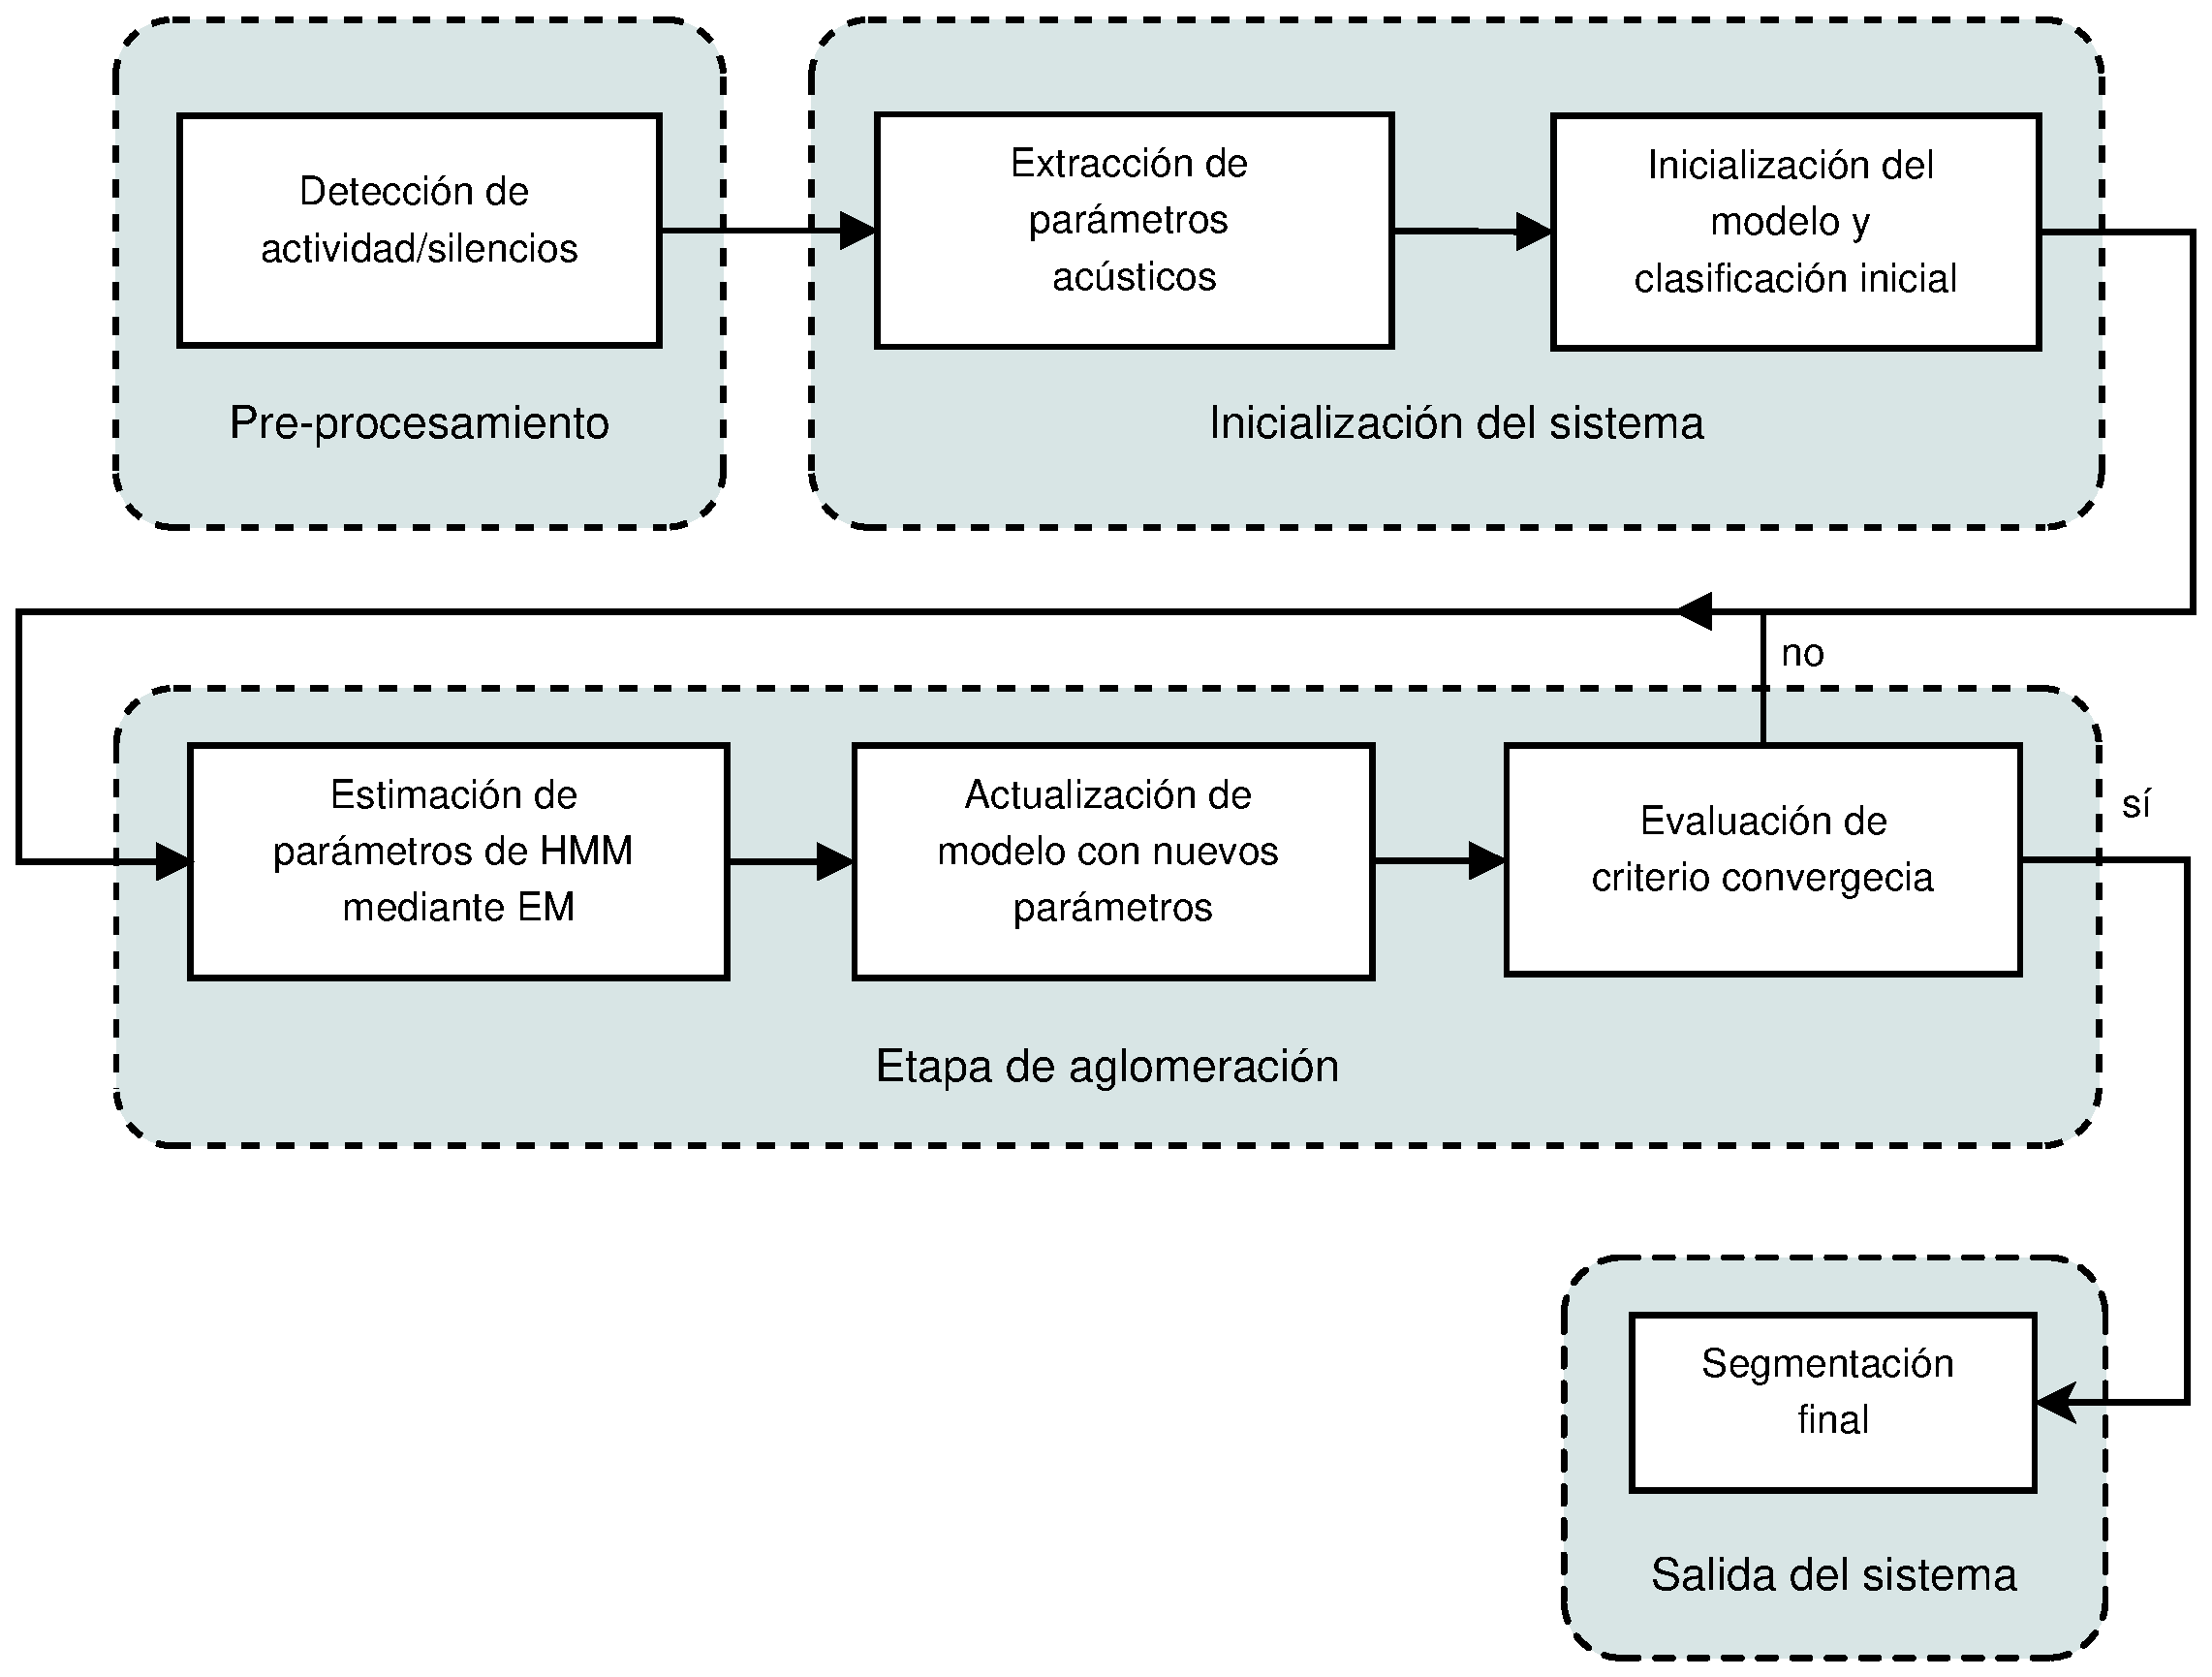
\includegraphics[width=0.8\textwidth]{gfx/ASR_flow}
  \end{center}
\end{frame}

\subsection{Procesamiento acústico}

\begin{frame}{Procesamiento acústico}{Pre-procesamiento de la señal}
%{Elminación de ruido / Detección de silencios}
  \small {
  \vspace{0mm} 
  \begin{columns} 
    \begin{column}{0.6\textwidth} 
      \hfill 
      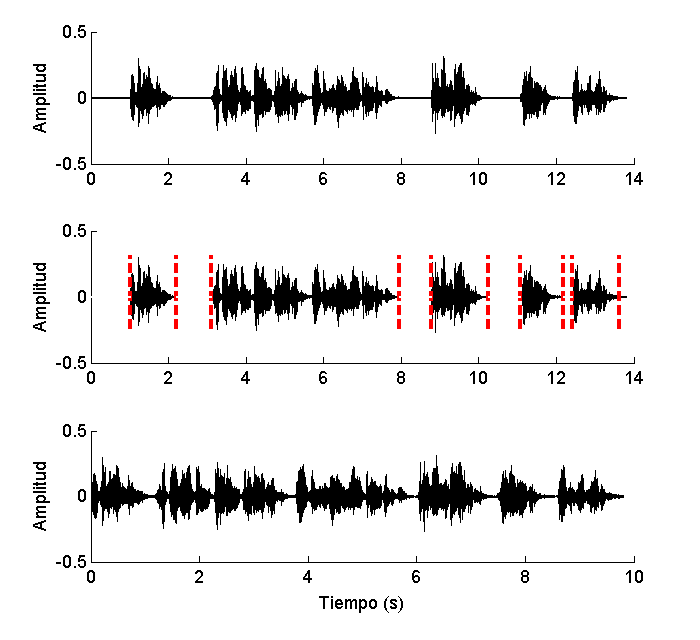
\includegraphics[width=0.9\textwidth]{gfx/filename51}
    \end{column}
    \begin{column}{0.4\textwidth}
      \vspace{-8mm}
      \begin{itemize}
        \setlength{\itemindent}{-2em}      
        \itemsep 4.6em    
        \item Señal original
        \item Identificación de silencios (SAD)
        \item Señal de audio recortada
      \end{itemize}
    \end{column}   
  \end{columns}   
  }
\end{frame}

%\subsubsection{Obtención de vector de características}

\begin{frame}{Procesamiento acústico}{Obtención de vectores característicos (I)}
  \small {
  \vspace{0mm} 
  \begin{columns}   
    \begin{column}{0.6\textwidth} 
      \hfill  
      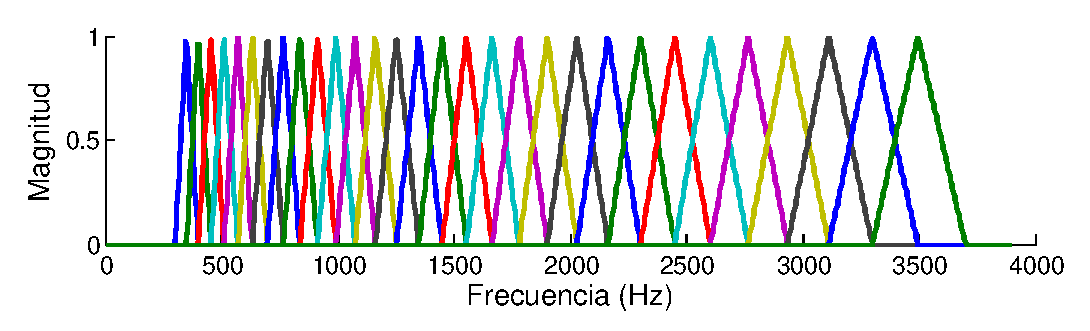
\includegraphics[width=0.9\textwidth]{gfx/example_mfcc}    
    \end{column}
    \begin{column}{0.4\textwidth}
      \vspace{-8mm} 
      \begin{itemize}
        \setlength{\itemindent}{-2em}      
        \itemsep 4.6em    
        \item Banco de filtros
      \end{itemize}
    \end{column}   
  \end{columns}   
  }
  \vspace{1.5em}
  \begin{itemize}
    \itemsep1em
    \item Se utilizará un banco de filtros (usualmente triangulares) espaciados en la escala~Mel. 

    \item Se puede calcular de la siguiente manera:~~ $m = 2595 \cdot \log_{10} \left(1 + \dfrac{f}{700}\right)$

    \item Hay varios parámetros al momento diseñar el banco: número de filtros, frecuencia mínima y máxima, así como el ancho de banda de cada filtro.
  \end{itemize}
\end{frame}

\begin{frame}{Procesamiento acústico}{Obtención de vectores característicos (II)}
  \small {
  \vspace{0mm} 
  \begin{columns}   
    \begin{column}{0.6\textwidth} 
      \hfill  
      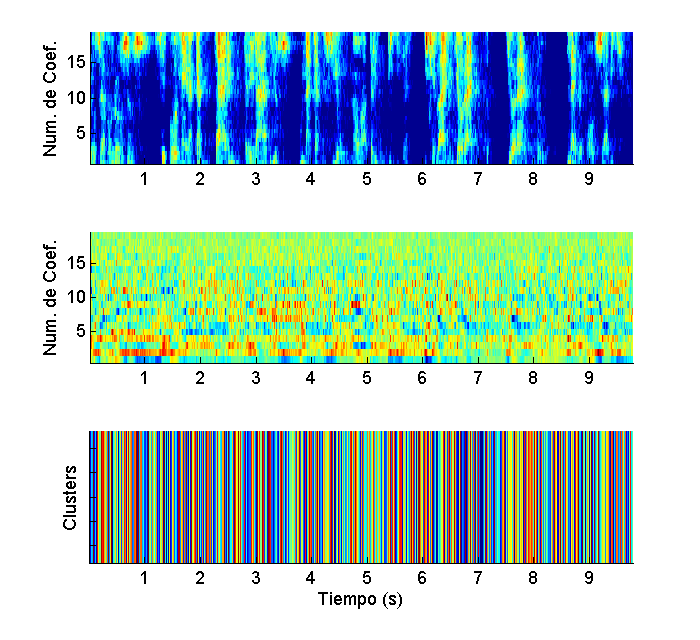
\includegraphics[width=0.9\textwidth]{gfx/filename52}    
    \end{column}
    \begin{column}{0.4\textwidth}
      \vspace{-8mm} 
      \begin{itemize}
        \setlength{\itemindent}{-2em}      
        \itemsep 4.6em    
        \item FFT + FilterBank + log(POW)
        \item DCT
        \item k-means++
      \end{itemize}
    \end{column}   
  \end{columns}   
  }
\end{frame}